%chktex-file 46
%chktex-file 21
%chktex-file 3
%chktex-file 13
%chktex-file 8
%chktex-file 25

This section presents a comprehensive discussion of the results obtained from the application of the eBN framework, addressing the relevant uncertainties in the concrete corrosion process, with a particular focus on imprecise data arising from climate change projections. Before delving into these findings, we first summarize the outcomes of the sensitivity analysis (SA) performed on the carbonation-induced and chloride-induced corrosion processes.

\subsection{Sensitivity Analysis of concrete corrosion process models}
SA has been perfomed to identify the most influential factors affecting concrete corrosion processes.
% SA is vital for the efficiency of a probabilistic risk assessment tool, as it enables the exclusion of variables with minimal impact on outcomes, thereby reducing the computational demands of the risk assessment framework.
Sobol's indices are used as robust and reliable indicators for global SA. 
This choice is justified because of their rigorous theoretical foundation in variance-based decomposition, the ability to capture both linear and nonlinear dependencies, including high-order interactions among random variables and the clear interpretability~\cite{Sobols_indices_SOBOL}.
Sobol's indices have been evaluated for both corrosion models to rank the effect of the random variables on the respective outputs. 

\subsubsection{Carbonation-induced corrosion}\label{SA_carbonation}
The random variables considered in the SA of the carbonation model are the same as those introduced in Sec.~\ref{ebn_chloride_section}. 
The variables \textit{Ce}, \textit{Ca}, \textit{k\_site}, \textit{n\_d}, \textit{n\_m}, \textit{E}, \textit{ratio\_wc} and \textit{D\_i} follow the same probability distribution across all decades and climatic projections, whereas the distributions of \textit{T}, \textit{ppm\_CO\textsubscript{2}} and \textit{RH\_int} vary depending on the decade and climate projection. \\ 
Figure~\ref{Sobol_carb_2020ssp1} shows the Sobol's indices for the carbonation model during the first decade under the \textit{ssp1} climate scenario. 
Both the first-order and total-effect Sobol' indices are negligible for all input variables except for relative humidity, indicating that \textit{RH\_int} is the only variable that significantly contributes to the output variance, both independently (first-order effect) and through interactions with other variables (total effect).
Sobol's indices have been computed for each decade and for all considered climate projections. The results consistently exhibit the same trend as illustrated for the first-decade and \textit{ssp1} projection, with relative humidity remaining the dominant factor influencing output variance. 

\begin{figure}[H]
    \centering
    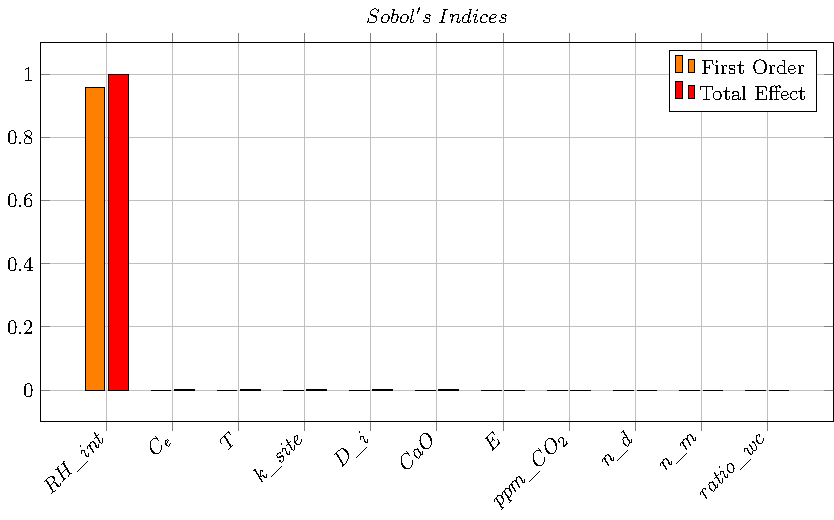
\includegraphics[width=0.8\linewidth]{imgs/pdfs/sobols_indices/carbonation/17_1_sobols_2020_ssp1.pdf}
    \caption{Sobol's indices of the model for carbonation-induced corrosion considering the random variables identified by the year 2020 and the projection \textit{ssp1}}\label{Sobol_carb_2020ssp1}
\end{figure}
In Fig.~\ref{Sobol_carb_2020uniform}, Sobol's indices are presented under the assumption that all input variables follow uniform probability distributions. For the variables \textit{Ce}, \textit{Ca}, \textit{k\_site}, \textit{n\_d}, \textit{n\_m}, \textit{E}, \textit{ratio\_wc}, and \textit{D\_i}, the uniform distribution bounds were defined as the minimum and maximum values obtained from $10^4$ samples drawn from their respective original distributions. For the time-dependent variables \textit{T}, \textit{ppm\_CO\textsubscript{2}}, and \textit{RH\_int}, the uniform bounds for each decade were derived from the minimum and maximum of a merged set of $3 \times 10^4$ samples, aggregated across all climate change projections. This approach is adopted to enhance the potential influence of the distribution tails, particularly those of the original Gaussian distributions, thereby allowing a more comprehensive assessment of the input variables' impact on model output variability. 
The analysis confirms that relative humidity continues to exert the most significant influence on the variability of the model output, even under the assumption of uniformly distributed inputs.
\begin{figure}[H]
    \centering
    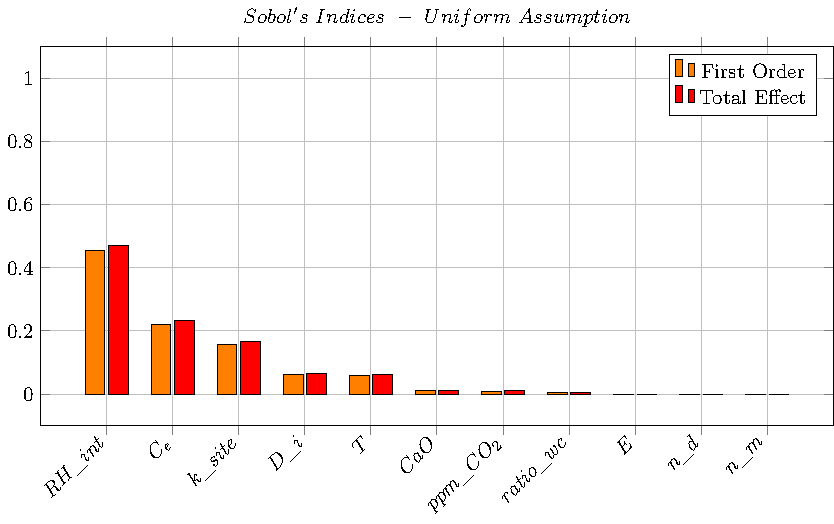
\includegraphics[width=0.8\linewidth]{imgs/pdfs/sobols_indices/carbonation/16_1_sobols_uniform_2020.pdf}
    \caption{Sobol's indices of the model for carbonation-induced corrosion at year 2020 under the uniform distributions assumption}\label{Sobol_carb_2020uniform}
\end{figure}

\subsubsection{Carbonation-induced corrosion}
The same procedure presented in Sec.~\ref{SA_carbonation} has been applied to the chloride-induced corrosion model, obtaining the results presented in Fig.~\ref{Sobol_ch_2020ssp1} and Fig.~\ref{Sobol_ch_2020uniform}.
\begin{figure}[H]
    \centering
    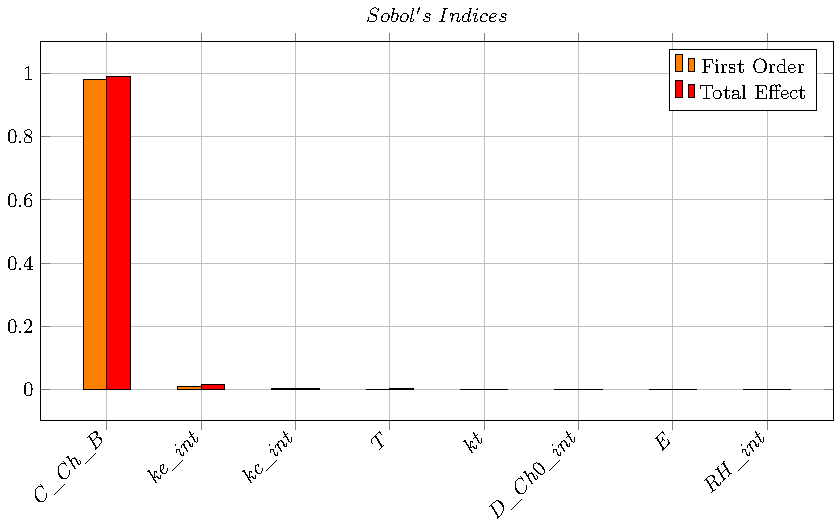
\includegraphics[width=0.8\linewidth]{imgs/pdfs/sobols_indices/chloride/19_1_sobols_withRH_2020_ssp1.pdf}
    \caption{Sobol's indices of the model for chloride-induced corrosion considering the random variables identified by the year 2020 and the projection \textit{ssp1}}\label{Sobol_ch_2020ssp1}
\end{figure}

\begin{figure}[H]
    \centering
    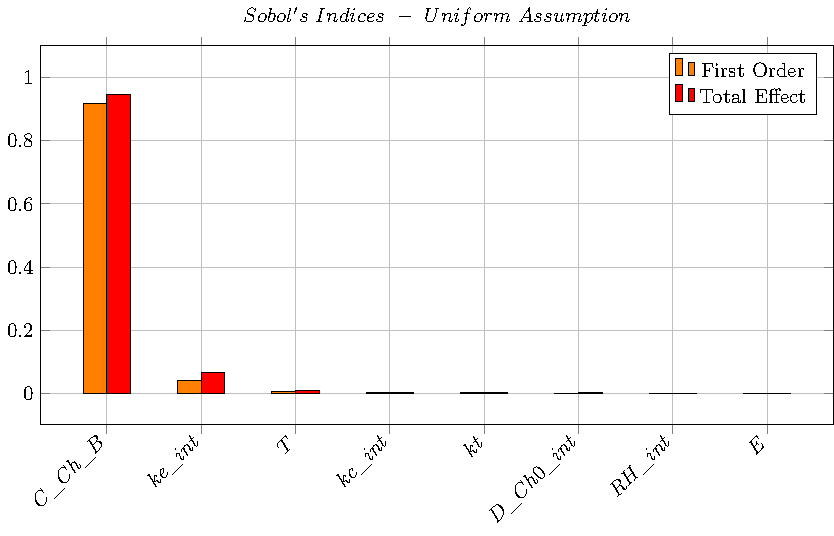
\includegraphics[width=0.8\linewidth]{imgs/pdfs/sobols_indices/chloride/18_1_sobols_withRH_uniform_2020.pdf}
    \caption{Sobol's indices of the model for chloride-induced corrosion at year 2020 under the uniform distributions assumption}\label{Sobol_ch_2020uniform}
\end{figure}
For the chloride-induced corrosion model, relative humidity is identified as the primary driver of output variability in both distributional scenarios. However, under the uniform input assumption, additional factors such as temperature, the curing factor and the environmental factor also exhibit a non-negligible influence on the output variance.

\subsection{Exceedance Probabilities for Corrosion}

The results of the SA motivated the introduction of two control nodes, \textit{DeH} and \textit{DeCh}, to regulate relative humidity and chloride concentration at the system boundaries. 
These nodes are defined as follows.
The node \textit{DeH} represents a dehumidifier unit, modelled as a root node with a failure probability of $10^{-4}$ and is parent to both the model nodes.
Its influence is identical across the two models: when operational (i.e., not in a failed state) and when the relative humidity exceeds a specified threshold, it reduces the humidity to a defined target level. 
In the eBN described in Sec.~\ref{caseofstudy}, the threshold and target relative humidity values are set to 0.25 and 0.2, respectively.
The node \textit{DeCh} is conceptually similar to \textit{DeH}.
It is also a root node with a failure probability of $10^{-4}$ and is defined by a threshold and target value for chloride concentration. 
Unlike \textit{DeH}, \textit{DeCh} influences only the chloride-induced corrosion model, where it acts to reduce the chloride concentration at the system boundary when the threshold is exceeded. 
In the eBN presented in Sec.~\ref{caseofstudy}, the threshold and target chloride concentration values are 0.9 and 0.7, respectively.\\

\subsubsection{Precise eBN}
Exceedance probabilities for corrosion are contained in the CPTs of the two functional of the eBNs presented in Sec.\ref{caseofstudy}. 
Results for the precise eBN depicted in Fig.~\ref{fig:precise_ebn} are obtained through Monte Carlo simulation with $10^4$ samples and considering a maximum allowed carbonation depth of \SI{3}{\centi\meter} and a maximum allowed chloride penetration of \SI{12}{\centi\meter}, where the chloride penetration is defined as the depth when chloride concentration is larger than \SI{0.9}{\kilogram\per\cubic\meter}, for defining the performance functions of nodes \textit{carb_depth} and \textit{ch_corr_depth}.
In particular the CPT of the carbonation node in the precise rBN depicted in Fig.\ref{fig:precise_rbn} has 54 possible scenarios, identified by 9 decades, 3 projections and 2 possible states of the dehumidifier unit. This CPT shows that whenever the dehumidifier unit is working the carbonation process never reaches the failure threshold, for all the decades before year 2060 the failure never occurs, and after year 2060 failure of the system can take place with the probabilities shown in Tab.~\ref{Carbonation_precise_cpt}.

\begin{table}[H]
    \begin{center}
    \caption{Carbonation-induced corrosion node partial CPT for the precise eBN of Fig.~\ref{carbonation_ebn}}\label{Carbonation_precise_cpt}
        \begin{tabular}{P{6cm}P{4cm}}
            \toprule
            \textbf{scenarios} & \textbf{states probabilities} \\
            \midrule
                \begin{tabular}{P{1.5cm}P{1.5cm}P{1.5cm}}
                    \textbf{t} & \textbf{DeH} & \textbf{proj} \\
                    \midrule
                    2060 & failed & ssp1 \\
                    2060 & failed & ssp2 \\
                    2060 & failed & ssp5 \\
                    2070 & failed & ssp1 \\
                    2070 & failed & ssp2 \\
                    2070 & failed & ssp5 \\
                    2080 & failed & ssp1 \\
                    2080 & failed & ssp2 \\
                    2080 & failed & ssp5 \\
                    2090 & failed & ssp1 \\
                    2090 & failed & ssp2 \\
                    2090 & failed & ssp5 \\
                    2100 & failed & ssp1 \\
                    2100 & failed & ssp2 \\
                    2100 & failed & ssp5 \\
                \end{tabular} &
                \begin{tabular}{P{1.5cm}P{1.5cm}}
                    \textbf{failed} & \textbf{safe} \\
                    \midrule
                    0.0001 & 0.9999 \\
                    0.0012 & 0.9988 \\
                    0.0103 & 0.9897 \\
                    0.0056 & 0.9944 \\
                    0.0241 & 0.9759 \\
                    0.0991 & 0.9009 \\
                    0.0374 & 0.9626 \\
                    0.1110 & 0.8890 \\
                    0.3082 & 0.6918 \\
                    0.1232 & 0.8768 \\
                    0.2694 & 0.7306 \\
                    0.5290 & 0.4710 \\
                    0.2570 & 0.7430 \\
                    0.4630 & 0.5370 \\
                    0.7075 & 0.2925 \\
                \end{tabular} \\
        \end{tabular}
    \end{center}
\end{table}

The CPT of the chloride-induced corrosion node in the precise rBN depicted in Fig.\ref{fig:precise_rbn} has 108 possible scenarios, identified by 9 decades, 3 projections, 2 possible states of the dehumidifier unit and 2 possible states for node \textit{DeCh}. 
This CPT shows that whenever the unit to reduce the chloride concentration at system boundary is working, the chloride-induced corrosion process never reaches the failure threshold. 
Some of the remaining scenarios are shown in Tab.~\ref{Chloride_precise_cpt}.

\begin{table}[H]
    \begin{center}
    \caption{Carbonation-induced corrosion node partial CPT for the precise eBN of Fig.~\ref{carbonation_ebn}}\label{Chloride_precise_cpt}
        \begin{tabular}{P{7cm}P{4cm}}
            \toprule
            \textbf{scenarios} & \textbf{states probabilities} \\
            \midrule
                \begin{tabular}{P{1.2cm}P{1.3cm}P{1.3cm}P{1.2cm}}
                    \textbf{t} & \textbf{DeH} & \textbf{DeCh} & \textbf{proj} \\
                    \midrule
                    2020 & failed & failed & ssp1 \\
                    2020 & failed & failed & ssp2 \\
                    2020 & failed & failed & ssp5 \\
                    2020 & working & failed & ssp1 \\
                    2020 & working & failed & ssp2 \\
                    2020 & working & failed & ssp5 \\
                    2030 & failed & failed & ssp1 \\
                    2030 & failed & failed & ssp2 \\
                    2030 & failed & failed & ssp5 \\
                    2030 & working & failed & ssp1 \\
                    2030 & working & failed & ssp2 \\
                    2030 & working & failed & ssp5 \\
                    2040 & failed & failed & ssp1 \\
                    2040 & failed & failed & ssp2 \\
                    2040 & failed & failed & ssp5 \\
                    2040 & working & failed & ssp1 \\
                    2040 & working & failed & ssp2 \\
                    2040 & working & failed & ssp5 \\
                    \dots & \dots & \dots & \dots \\
                    % 2050 & failed & failed & ssp1 \\
                    % 2050 & failed & failed & ssp2 \\
                    % 2050 & failed & failed & ssp5 \\
                    % 2050 & working & failed & ssp1 \\
                    % 2050 & working & failed & ssp2 \\
                    % 2050 & working & failed & ssp5 \\
                    % 2060 & failed & failed & ssp1 \\
                    % 2060 & failed & failed & ssp2 \\
                    % 2060 & failed & failed & ssp5 \\
                    % 2060 & working & failed & ssp1 \\
                    % 2060 & working & failed & ssp2 \\
                    % 2060 & working & failed & ssp5 \\
                    % 2070 & failed & failed & ssp1 \\
                    % 2070 & failed & failed & ssp2 \\
                    % 2070 & failed & failed & ssp5 \\
                    % 2070 & working & failed & ssp1 \\
                    % 2070 & working & failed & ssp2 \\
                    % 2070 & working & failed & ssp5 \\
                    % 2080 & failed & failed & ssp1 \\
                    % 2080 & failed & failed & ssp2 \\
                    % 2080 & failed & failed & ssp5 \\
                    % 2080 & working & failed & ssp1 \\
                    % 2080 & working & failed & ssp2 \\
                    % 2080 & working & failed & ssp5 \\
                    2090 & failed & failed & ssp1 \\
                    2090 & failed & failed & ssp2 \\
                    2090 & failed & failed & ssp5 \\
                    2090 & working & failed & ssp1 \\
                    2090 & working & failed & ssp2 \\
                    2090 & working & failed & ssp5 \\
                    2100 & failed & failed & ssp1 \\
                    2100 & failed & failed & ssp2 \\
                    2100 & failed & failed & ssp5 \\
                    2100 & working & failed & ssp1 \\
                    2100 & working & failed & ssp2 \\
                    2100 & working & failed & ssp5 \\
                \end{tabular} &
                \begin{tabular}{P{1.5cm}P{1.5cm}}
                    \textbf{failed} & \textbf{safe} \\
                    \midrule
                    0.0045 & 0.9955 \\
                    0.0054 & 0.9945 \\
                    0.0043 & 0.9957 \\
                    0.0021 & 0.9979 \\
                    0.0016 & 0.9984 \\
                    0.0021 & 0.9979 \\
                    0.0462 & 0.9538 \\
                    0.0445 & 0.9555 \\
                    0.0470 & 0.9530 \\
                    0.0291 & 0.9709 \\
                    0.0279 & 0.9721 \\
                    0.0301 & 0.9699 \\
                    0.1159 & 0.8841 \\
                    0.1179 & 0.8821 \\
                    0.1266 & 0.8734 \\
                    0.0862 & 0.9138 \\
                    0.0911 & 0.9089 \\
                    0.0975 & 0.9025 \\
                    \dots & \dots \\
                    % 0.1781 & 0.8219 \\
                    % 0.1819 & 0.8181 \\
                    % 0.1929 & 0.8071 \\
                    % 0.1472 & 0.8528 \\
                    % 0.1501 & 0.8499 \\
                    % 0.1596 & 0.8404 \\
                    % 0.2431 & 0.7569 \\
                    % 0.2464 & 0.7536 \\
                    % 0.2667 & 0.7333 \\
                    % 0.1962 & 0.8038 \\
                    % 0.2139 & 0.7861 \\
                    % 0.2216 & 0.7784 \\
                    % 0.2800 & 0.7200 \\
                    % 0.2819 & 0.7181 \\
                    % 0.3082 & 0.6918 \\
                    % 0.2483 & 0.7517 \\
                    % 0.2512 & 0.7488 \\
                    % 0.2774 & 0.7226 \\
                    % 0.3137 & 0.6863 \\
                    % 0.3337 & 0.6663 \\
                    % 0.3594 & 0.6406 \\
                    % 0.2816 & 0.7184 \\
                    % 0.2925 & 0.7075 \\
                    % 0.3140 & 0.6860 \\
                    0.3361 & 0.6639 \\
                    0.3711 & 0.6289 \\
                    0.3884 & 0.6116 \\
                    0.3052 & 0.6948 \\
                    0.3314 & 0.6686 \\
                    0.3577 & 0.6423 \\
                    0.3510 & 0.6490 \\
                    0.3771 & 0.6229 \\
                    0.4194 & 0.5806 \\
                    0.3250 & 0.6750 \\
                    0.3616 & 0.6384 \\
                    0.3828 & 0.6172 \\
                \end{tabular} \\
        \end{tabular}
    \end{center}
\end{table}

\subsubsection{Imprecise eBN}
Results for the imprecise eBN depicted in Fig.~\ref{fig:imprecise_ebn} are obtained through standard Double Loop simulation with an inner Monte Carlo simulation with $10^3$ samples. 
Performance functions of the two corrosion model nodes are defined in the same way as for the precise eBN.
The CPT of the carbonation node in the imprecise rBN depicted in Fig.\ref{fig:imprecise_rbn} still has 54 possible scenarios, still never reaches the failure threshold whenever the dehumidifier unit is working the carbonation process and for all the decades before year 2050. Failure probability intervals after year 2050 are shown in Tab.~\ref{Carbonation_imprecise_cpt}.

\begin{table}[H]
    \begin{center}
    \caption{Carbonation-induced corrosion node partial CPT for the precise eBN of Fig.~\ref{carbonation_ebn}}\label{Carbonation_imprecise_cpt}
        \begin{tabular}{P{5cm}P{6cm}}
            \toprule
            \textbf{scenarios} & \textbf{states probabilities} \\
            \midrule
                \begin{tabular}{P{0.8cm}P{1.2cm}P{0.8cm}}
                    \textbf{t} & \textbf{DeH} & \textbf{proj} \\
                    \midrule
                    2050 & failed & ssp1 \\
                    2050 & failed & ssp2 \\
                    2050 & failed & ssp5 \\
                    2060 & failed & ssp1 \\
                    2060 & failed & ssp2 \\
                    2060 & failed & ssp5 \\
                    2070 & failed & ssp1 \\
                    2070 & failed & ssp2 \\
                    2070 & failed & ssp5 \\
                    2080 & failed & ssp1 \\
                    2080 & failed & ssp2 \\
                    2080 & failed & ssp5 \\
                    2090 & failed & ssp1 \\
                    2090 & failed & ssp2 \\
                    2090 & failed & ssp5 \\
                    2100 & failed & ssp1 \\
                    2100 & failed & ssp2 \\
                    2100 & failed & ssp5 \\
                \end{tabular} &
                \begin{tabular}{P{2.5cm}P{2.5cm}}
                    \textbf{failed} & \textbf{safe} \\
                    \midrule
                    $[0.0; 0.0]$          &  $[1.0; 1.0]$\\
                    $[0.0; 4.76e^{-4}]$   &  $[0.999524; 1.0]$\\
                    $[0.0; 0.001]$        &  $[0.999; 1.0]$\\
                    $[1.73e^{-6}; 0.002]$ &  $[0.998; 0.999998]$\\
                    $[2.50e^{-4}; 0.007]$ &  $[0.993; 0.99975]$\\
                    $[0.0; 0.037]$        &  $[0.963; 1.0]$\\
                    $[0.0;  0.027]$       &  $[0.973; 1.0]$\\
                    $[0.001; 0.073]$      &  $[0.927; 0.999]$\\
                    $[0.033; 0.195]$      &  $[0.805; 0.967]$\\
                    $[0.005; 0.081]$      &  $[0.919; 0.995]$\\
                    $[0.034; 0.212]$      &  $[0.788; 0.966]$\\
                    $[0.183; 0.407]$      &  $[0.593; 0.817]$\\
                    $[0.036; 0.249]$      &  $[0.751; 0.964]$\\
                    $[0.137; 0.369]$      &  $[0.631; 0.863]$\\
                    $[0.384; 0.601]$      &  $[0.399; 0.616]$\\
                    $[0.157; 0.426]$      &  $[0.574; 0.843]$\\
                    $[0.285; 0.614]$      &  $[0.386; 0.715]$\\
                    $[0.575; 0.745]$      &  $[0.255; 0.425]$\\
                \end{tabular} \\
        \end{tabular}
    \end{center}
\end{table}

As for the precise BN, the CPT of the chloride-induced corrosion node in the precise rBN depicted in Fig.\ref{fig:imprecise_rbn} has 108 possible scenarios and whenever the unit to reduce the chloride concentration at system boundary is working, the chloride-induced corrosion process never reaches the failure threshold. 
Some of the remaining scenarios are shown in Tab.~\ref{Chloride_imprecise_cpt}.
\begin{table}[H]
    \begin{center}
    \caption{Carbonation-induced corrosion node partial CPT for the precise eBN of Fig.~\ref{carbonation_ebn}}\label{Chloride_imprecise_cpt}
        \begin{tabular}{P{5.2cm}P{6cm}}
            \toprule
            \textbf{scenarios} & \textbf{states probabilities} \\
            \midrule
                \begin{tabular}{P{0.6cm}P{1.3cm}P{1.3cm}P{0.7cm}}
                    \textbf{t} & \textbf{DeH} & \textbf{DeCh} & \textbf{proj} \\
                    \midrule
                    2020 & failed & failed & ssp1 \\
                    2020 & failed & failed & ssp2 \\
                    2020 & failed & failed & ssp5 \\
                    2020 & working & failed & ssp1 \\
                    2020 & working & failed & ssp2 \\
                    2020 & working & failed & ssp5 \\
                    2030 & failed & failed & ssp1 \\
                    2030 & failed & failed & ssp2 \\
                    2030 & failed & failed & ssp5 \\
                    2030 & working & failed & ssp1 \\
                    2030 & working & failed & ssp2 \\
                    2030 & working & failed & ssp5 \\
                    2040 & failed & failed & ssp1 \\
                    2040 & failed & failed & ssp2 \\
                    2040 & failed & failed & ssp5 \\
                    2040 & working & failed & ssp1 \\
                    2040 & working & failed & ssp2 \\
                    2040 & working & failed & ssp5 \\
                    \dots & \dots & \dots & \dots \\
                    2090 & failed & failed & ssp1 \\
                    2090 & failed & failed & ssp2 \\
                    2090 & failed & failed & ssp5 \\
                    2090 & working & failed & ssp1 \\
                    2090 & working & failed & ssp2 \\
                    2090 & working & failed & ssp5 \\
                    2100 & failed & failed & ssp1 \\
                    2100 & failed & failed & ssp2 \\
                    2100 & failed & failed & ssp5 \\
                    2100 & working & failed & ssp1 \\
                    2100 & working & failed & ssp2 \\
                    2100 & working & failed & ssp5 \\
                \end{tabular} &
                \begin{tabular}{P{2.5cm}P{2.5cm}}
                    \textbf{failed} & \textbf{safe} \\
                    \midrule
                    $[0.0, 0.018]$ & $[0.982, 1.0]$ \\
                    $[0.0, 0.02]$ & $[0.98, 1.0]$ \\
                    $[0.0, 0.024]$ & $[0.976, 1.0]$ \\
                    $[6.17e^{-5}, 0.01]$ & $[0.99, 0.9993]$ \\
                    $[0.000437, 0.015]$ & $[0.985, 0.999563]$ \\
                    $[4.55e^{-5}, 0.012]$ & $[0.988, 0.99995]$ \\
                    $[0.016, 0.099]$ & $[0.901, 0.984]$ \\
                    $[0.015, 0.098]$ & $[0.902, 0.985]$ \\
                    $[0.0140, 0.094]$ & $[0.906, 0.9860]$ \\
                    $[0.008, 0.072]$ & $[0.928, 0.992]$ \\
                    $[0.003, 0.068]$ & $[0.932, 0.997]$ \\
                    $[0.004, 0.07]$ & $[0.93, 0.996]$ \\
                    $[0.0640, 0.165]$ & $[0.835, 0.936]$ \\
                    $[0.058, 0.192]$ & $[0.808, 0.942]$ \\
                    $[0.064, 0.193]$ & $[0.807, 0.936]$ \\
                    $[0.041, 0.106]$ & $[0.894, 0.959]$ \\
                    $[0.042, 0.16]$ & $[0.84, 0.958]$ \\
                    $[0.036, 0.113]$ & $[0.887, 0.964]$ \\
                    \dots & \dots \\
                    $[0.261, 0.442]$ & $[0.558, 0.739]$ \\
                    $[0.272, 0.426]$ & $[0.574, 0.728]$ \\
                    $[0.319, 0.45]$ & $[0.55, 0.681]$ \\
                    $[0.231, 0.404]$ & $[0.596, 0.769]$ \\
                    $[0.247, 0.388856]$ & $[0.611144, 0.753]$ \\
                    $[0.272, 0.423]$ & $[0.577, 0.728]$ \\
                    $[0.286, 0.403]$ & $[0.597, 0.714]$ \\
                    $[0.299, 0.425845]$ & $[0.574155, 0.701]$ \\
                    $[0.354, 0.495]$ & $[0.505, 0.646]$ \\
                    $[0.258, 0.391]$ &  $[0.609, 0.742]$ \\
                    $[0.276, 0.404]$ & $[0.596, 0.724]$ \\
                    $[0.303, 0.46]$ & $[0.54, 0.697]$ \\
                \end{tabular} \\
        \end{tabular}
    \end{center}
\end{table}

\subsubsection{Results comparison}
In this section, results regarding the threshold exceedance probability for the two nodes related to carbonation-induced and chloride-induced corrosion, and coming from the precise and the imprecise eBN are compared. 
In particular, as expected, it is possible to see that in all the analysed cases of Figs.~\ref{comparizon_carb},~\ref{comparizon_ch_brokenbroken} and~\ref{comparizon_ch_brokenworking}, failure probability intervals always contain the crisp failure probability values coming from the precise eBN.
\begin{figure}[H]
    \centering
    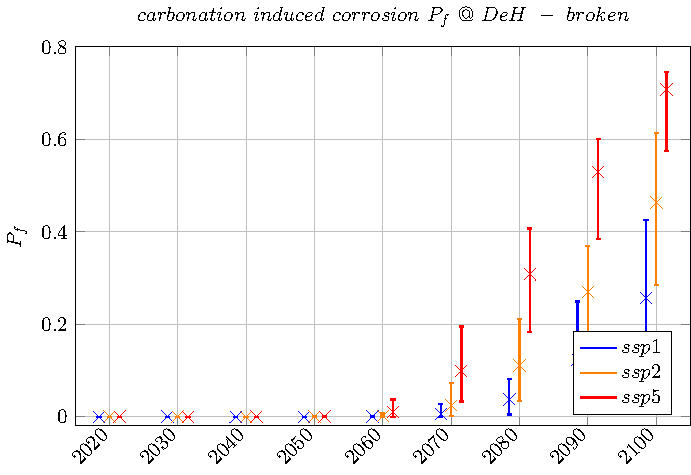
\includegraphics[width=0.8\linewidth]{imgs/pdfs/22_carbonation_comparizon_broken.pdf}
    \caption{Exceedance probabilities comparison between precise and imprecise eBN for carbonation-induced corrosion node and scenarios when the \textit{DeH} is failed}\label{comparizon_carb}
\end{figure}

\begin{figure}[H]
    \centering
    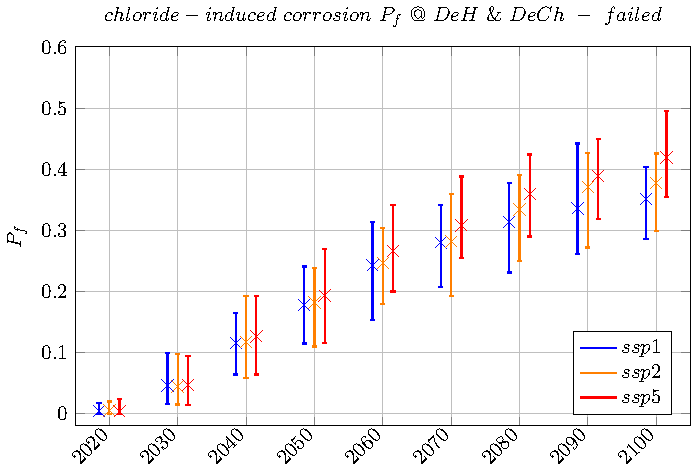
\includegraphics[width=0.8\linewidth]{imgs/pdfs/20_Chloride_comparizon_brokenbroken.pdf}
    \caption{Exceedance probabilities comparison between precise and imprecise eBN for chloride-induced corrosion node and scenarios when both \textit{DeH} and \textit{DeCh} are failed}\label{comparizon_ch_brokenbroken}
\end{figure}

\begin{figure}[H]
    \centering
    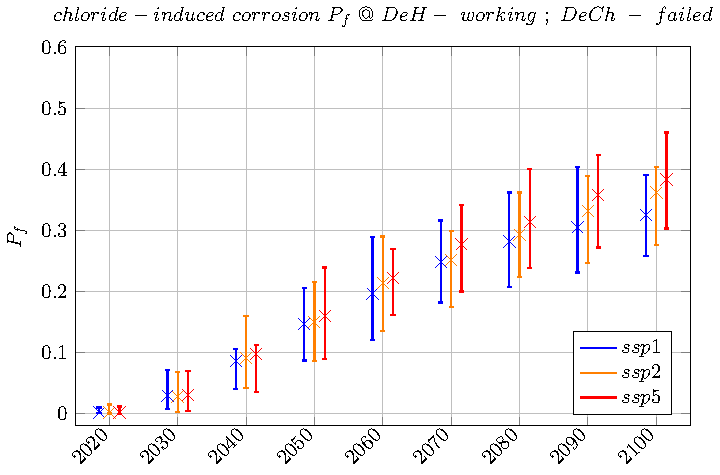
\includegraphics[width=0.8\linewidth]{imgs/pdfs/21_Chloride_comparizon_workingbroken.pdf}
    \caption{Exceedance probabilities comparison between precise and imprecise eBN for chloride-induced corrosion node and scenarios when \textit{DeH} is working and \textit{DeCh} is failed}\label{comparizon_ch_brokenworking}
\end{figure}
